\documentclass[12pt,a4paper]{article}
\usepackage[utf8]{inputenc}
\usepackage[margin=2.5cm]{geometry}
\usepackage[slovene,english]{babel}
\usepackage[unicode,
    pdftex,
    pdfauthor={Erazem Kokot},
    pdftitle={Statisticna obdelava podatkov},
    pdfkeywords={verjetnost, statistika, obdelava podatkov},
    pdfsubject={Verjetnost in Statistika}]{hyperref}
\usepackage[justification=centering]{caption}
\usepackage{
    lipsum,
    graphicx,
    amsmath,
    amssymb,
    color,
    subcaption,
    fancyhdr,
    multicol
}

\captionsetup[figure]{name=Graf}
\inputencoding{utf8}

\title{Primer statistične obdelave podatkov:\\ Telesna in možganska teža sesalcev}
\author{Erazem Kokot}
\date{2020}

\setcounter{tocdepth}{2}

\begin{document}

    \begin{titlepage}
        \maketitle

        \vfill
        \begin{center}
            Fakulteta za Računalništvo in Informatiko

            Verjetnost in Statistika
        \end{center}
        \thispagestyle{empty}
    \end{titlepage}
    
    \selectlanguage{slovene}

    \tableofcontents

    \renewcommand{\listtablename}{Kazalo tabel}
    \listoftables

    \renewcommand{\listfigurename}{Kazalo grafov}
    \listoffigures
    \thispagestyle{empty}

    \newpage

    \section{Opis podatkov}


    \newpage
    \section{Opisna statistika}

Bonus točka V točki 2b) po Opisni statistiki, podajte razloge za transformacijo podatkov na
osnovi razsevnega diagrama, koeficienta korelacije in diagnostičnih grafov originalnih (netrans-
formiranih) podatkov. Potem pa nadaljujete z analizo v točkah 3-8.
    \newpage
    \subsection{Transformacija podatkov}

\begin{minipage}{0.45\textwidth}
    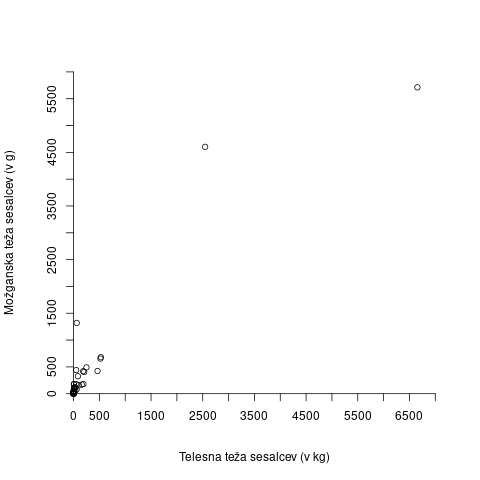
\includegraphics[width=1\textwidth]{res/netrans-razsevni-diagram.png}
    \captionof{figure}{Razsevni diagram\\(netransformiran)}
    \label{img:netrans-razsevni-diagram}
\end{minipage}
\hfill
\begin{minipage}{0.55\textwidth}
    Ob analizi razsevnega diagrama telesne teže sesalcev v primerjavi z velikostjo njihovih možganov
    (glej graf \ref{img:netrans-razsevni-diagram}) lahko opazimo, da podatki ne sledijo linearni zvezi.
    R ukaz \verb|(cor(mozgani$telteza, mozgani$moteza))|, ki izračuna korelacijski koeficient podanih spremenljivk,
    nam vrne rezultat \verb|[1] 0.9340911|, kar pomeni, da so podatki korelirani, tako da lahko vseeno nadaljujemo
    njihovo analizo, a jih moramo prvo transformirati.
    Podatke lahko transformiramo z logaritemsko funkcijo, pri čemer na razsevnem diagramu (glej graf \ref{img:razs-diag})
    opazimo, da so v tem primeru logaritmi podatkov linearno zvezni.
\end{minipage}
\\

Na grafu linearnosti modela (glej graf \ref{img:netrans-linearnost-modela}) je razvidno, da so točke zgoščene na levi
strani grafa, kar nakazuje na nelinearnost originalnega modela (pred transformacijo).

Na grafu normalnosti porazdelitve (glej graf \ref{img:netrans-normalnost-porazdelitve}) lahko opazimo odstopanja od
regresijske premice, a ne tako velika, da bi kazala na problem ujemanja podatkov z netransformiranim modelom.

Na grafu homogenosti variance (glej graf \ref{img:netrans-diagnosticni-grafi}) lahko opazimo, da so točke
zgoščene na levi strani, prav tako pa vidimo, da varianca naraste, zato zanjo ne moremo reči, da je homogena.

Na grafu vpliva točk na model (glej graf \ref{img:netrans-vpliv-tock-na-model}) lahko takoj opazimo tri točke z
največjo Cookovo razdaljo, 16., 29. in 30. podatkovno točko.

Da preverimo, če podatkovne točke zelo vplivajo na model, uporabimo spodnje ukaze:

\begin{verbatim}
    which(cooks.distance(model) > 4/57)
    any(cooks.distance(model)[c(16)] >= qf(0.5, 2, 57))
    any(cooks.distance(model)[c(29)] >= qf(0.5, 2, 57))
    any(cooks.distance(model)[c(30)] >= qf(0.5, 2, 57))
\end{verbatim}

pri čemer nam prvi ukaz vrne rezultat \emph{16, 29, 30}, zato smo zagnali tudi spodnje tri ukaze, kjer nam odgovora
za točki 16 in 30 vrneta rezultat \verb|[1] TRUE|, odgovor za točko 19 pa rezultat \verb|[1] FALSE|.
Ti rezultati nam povejo, da 16. in 30. podatkovna točka močno vplivata na linearnost modela, zato bi ju morali pred
nadaljevanjem odstraniti, a ker model na podlagi prejšnjih opažanj iz diagnostičnih grafov ne zadošča predpostavkam
linearnega modela, moramo podatke pred nadaljevanjem transformirati.

\newpage

\begin{figure}[h]
    \centering
    \begin{subfigure}[ht]{0.49\textwidth}
        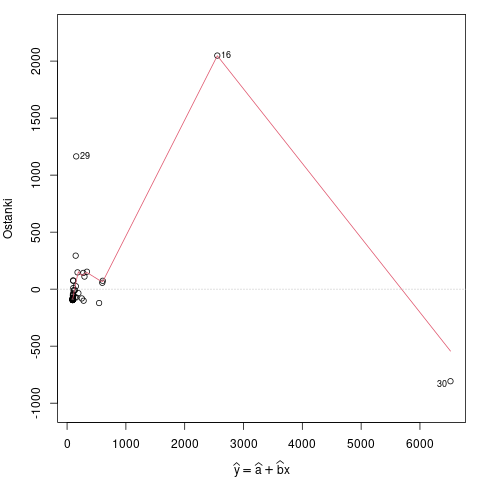
\includegraphics[width=1\textwidth]{res/netrans-linearnost-modela.png}
        \captionof{figure}{Linearnosti modela\\(netransformiran)}
        \label{img:netrans-linearnost-modela}
    \end{subfigure}
    \hfill
    \begin{subfigure}[ht]{0.49\textwidth}
        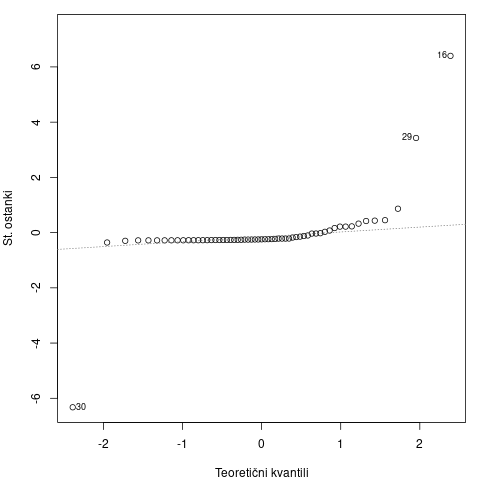
\includegraphics[width=1\textwidth]{res/netrans-normalnost-porazdelitve.png}
        \captionof{figure}{Normalnost porazdelitve\\(netransformiran)}
        \label{img:netrans-normalnost-porazdelitve}
    \end{subfigure}

    \begin{subfigure}[ht]{0.49\textwidth}
        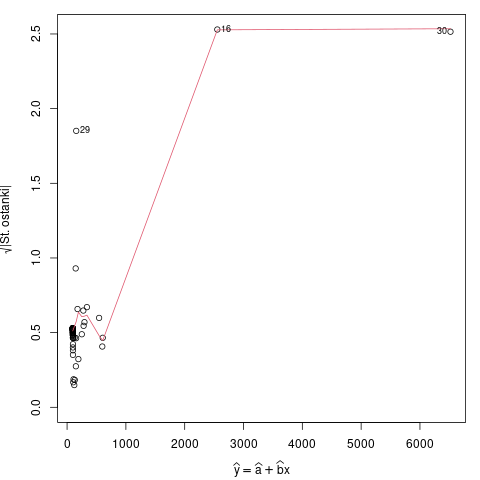
\includegraphics[width=1\textwidth]{res/netrans-homogenost-variance.png}
        \captionof{figure}{Homogenost variance\\(netransformiran)}
        \label{img:netrans-linearnost-modela}
    \end{subfigure}
    \hfill
    \begin{subfigure}[ht]{0.49\textwidth}
        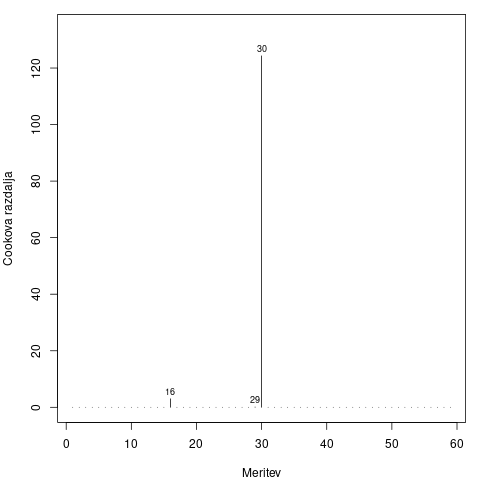
\includegraphics[width=1\textwidth]{res/netrans-vpliv-tock-na-model.png}
        \captionof{figure}{Vpliv točk na model\\(netransformiran)}
        \label{img:netrans-vpliv-tock-na-model}
    \end{subfigure}
    \caption{Netransformirani diagnostični grafi}
    \label{img:netrans-diagnosticni-grafi}
\end{figure}

Koda za generiranje diagnostičnih grafov je bolj podrobno predstavljena v poglavjih \ref{sec3} in \ref{sec5}.
    \newpage
    \section{Razsevni diagram in vzorčni koeficient korelacije}\label{sec3}

Prikažimo dobljene podatke na razsevnem diagramu:

\begin{figure}[h]
    \centering
    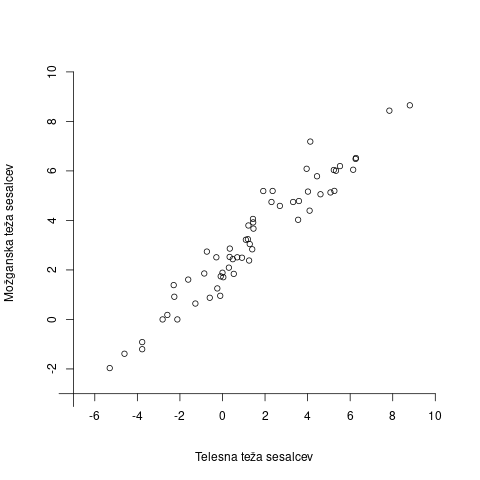
\includegraphics[scale=0.5]{res/razsevni-diagram.png}
    \caption{Razsevni diagram telesne in možganske teže sesalcev}
    \label{img:razs-diag}
\end{figure}

\noindent
Za izris grafa smo uporabili naslednjo R kodo:

\begin{verbatim}
    plot(
        x = log(mozgani$telteza),
        y = log(mozgani$mozteza),
        xlab = "Telesna teža sesalcev",
        ylab = "Možganska teža sesalcev",
        xlim = c(-7, 10),
        ylim = c(-3, 10),
        axes = FALSE
    )

    axis(1, pos = -3, at = seq(-8, 10, by = 2))
    axis(2, pos = -7, at = seq(-4, 10, by = 2))
\end{verbatim}

\newpage
Funkcija \verb|plot()| nam izriše razsevni diagram s podanimi parametri, v našem primeru z naslednjimi parametri:

\begin{itemize}
    \item \verb|x = log(mozgani$telteza)|, kjer \verb|x| predstavlja logaritemsko funkcijo telesne teže sesalcev,
    \item \verb|y = log(mozgani$mozteza)|, kjer \verb|y| predstavlja logaritemsko funkcijo možganske teže sesalcev,
    \item \verb|xlab| in \verb|ylab|, ki predstavljata ime x in y osi,
    \item \verb|xlim| in \verb|ylim|, ki določita začetne in končne koordinate x in y osi in
    \item \verb|axes = FALSE|, ki odstrani privzete koordinatne osi, saj jih želimo zamenjati z osmi, primernimi za
    naše parametre.
\end{itemize}

\noindent
Za izris koordinatnih osi uporabimo funkcijo \verb|axis()| s parametri \emph{1} ali \emph{2}, ki predstavljata
y in x os, \emph{pos}, ki predstavlja pozicijo postavitve osi, in \verb|at = seq()|, ki določi oznake na oseh
(s parametri \verb|seq(začetek, konec, razmak)|).
Moč korelacije lahko preverimo s \emph{Pearsonovim koeficientom}, kar v R naredimo z ukazom

\noindent
\verb|(r = cor(mozgani$telteza, mozgani$mozteza))|\label{en:r}, ki nam vrne rezultat \verb|[1] 0.9340911|.
Vrednost vzorčnega koeficienta korelacije je zelo visoka (r = 0.934), kar nakazuje visoko linearno povezanost
telesne teže sesalcev in teže njihovih možganov.
Ker je koeficient pozitiven nam to pove, da se z večjo telesno težo sesalca veča tudi teža njegovih možganov.
    \newpage
    \section{Formiranje linearnega regresijskega modela, prikaz računanja ocen naklona in odseka, ter enačba vzorčne regresijske premice}
    \newpage
    \section{Preverjanje predpostavk linearnega modela}
\subsection{Linearnost modela}
\subsection{Normalnost porazdelitve naključnih napak}
\subsection{Homogenost variance: graf in Breusch-Paganov test}
\subsection{Cookova razdalja: graf in analiza vpliva točk preko osnovnega pogoja, razsevnega diagrama in pogoja velikega vpliva}
    \newpage
    \section{Testiranje linearnosti modela in koeficient determinacije}

Poročilo o modelu lahko dobimo z ukazom \verb|summary(model)|, ki nam vrne spodnji (skrajšan) rezultat:

\begin{verbatim}
    Coefficients:
                Estimate Std. Error t value Pr(>|t|)    
    (Intercept)  2.17812    0.09487   22.96   <2e-16 ***
    lgtteza      0.74679    0.02773   26.93   <2e-16 ***
    ---
    Residual standard error: 0.6579 on 57 degrees of freedom
    Multiple R-squared:  0.9271,    Adjusted R-squared:  0.9259
    F-statistic: 725.4 on 1 and 57 DF,  p-value: < 2.2e-16
\end{verbatim}

Zanima nas samo testna statistika za testiranje linearnosti modela $T = 26.93$, z $df = 57$ prostorskimi
stopnjami, in p-vrednostjo $p = 2.2 \cdot 10^{16}$, ki je manjša od dane stopnje značilnosti 0.05.
S formalnim statističnim testiranjem smo potrdili, da linearni model ustreza podatkom.
Standardni odklon napak ocenjen s $S = 0.6579$, koeficient determinacije pa je enak $R^{2} = 0.9271$, kar je kvadrat
vzorčnega koeficienta korelacije. To pomeni, da 93\% variabilnosti telesne teže sesalcev pojasnjuje linearni regresijski
model.
    \newpage
    \section{Intervala zaupanja za naklon in odsek regresijske premice}

95\% interval zaupanja za neznani naklon in odsek regresijske premice lahko
izračunamo z ukazom \verb|round(confint(model), 3)|, ki nam vrne rezultat:

\begin{verbatim}
                2.5 % 97.5 %
    (Intercept) 1.988  2.368
    lgtteza     0.691  0.802
\end{verbatim}

Le-ta nam pove, da je interval zaupanja za odsek enak $I_{a} = [1.988, 2.368]$
in interval zaupanja za naklon enak $I_{b} = [0.691, 0.802]$.
    \newpage
    \section{Interval predikcije za vrednost Y pri izbrani vrednosti X}

Pri predvidevanju velikosti možganov sesalcev nas zanima bodoča vrednost spremenljivke Y (velikost možanov)
pri neki izbrani vrednosti spremenljivke X = $x_0$ (telesna teža).
Poleg predvidevane vrednosti $\widehat{y} = 95.8111 + 0.9653x_0$ za neke izbrane telesne teže sesalcev $x_0$ nas
zanimata tudi spodnja in zgornja meja, med katerima se nahaja velikost možganov sesalcev teh telesnih tež.
\emph{Interval predikcije} najdemo s pomočjo R funkcije \emph{predict()} in sicer z ukazoma
\verb|xteza = data.frame(telteza = c(100, 500, 2500))| in \verb|predict(model, xteza, interval = "predict")|,
ki nam vrne rezultate:

\begin{table}[h]
    \centering
    \begin{tabular}{cccc}
               & \textbf{fit} & \textbf{lwr} & \textbf{upr} \\
    \textbf{1} & 5.617202     & 4.277393     & 6.957011     \\
    \textbf{2} & 6.819109     & 5.464795     & 8.173424     \\
    \textbf{3} & 8.021017     & 6.646528     & 9.395506    
    \end{tabular}
    \caption{Interval predikcije}
    \label{tab:prediction}
\end{table}

\end{document}